% Section 6: Experimental Setup (SCOPAS dual-layer revision)

\section{Experimental Setup}
\label{sec:setup}

All experiments use the open SCOPAS framework (Radar, RF, EO, Acoustic) with dual-layer NSGA-II objectives \((M_{wp,coop}, M_{wp,noncoop}, \mathrm{cost})\) unless a split profile is stated. Sensor CapEx defaults: Radar \$50k, RF \$15k, EO \$25k, Acoustic \$8k, plus site activation \$15k.

\subsection{Synthetic city}

Scene: 1\,km$\times$1\,km, 196 buildings, 221 candidate sites (\texttt{data/examples/city\_10x10\_*}). Five critical assets define the threat map (Fig.~\ref{fig:scenario_city}). Airway altitudes \(\{20,45,65\}\)\,m. Paper rerun: resolution 30\,m, population 32, 18 generations, 4 cores (\texttt{configs/paper\_rerun\_city\_dual.json}).

\begin{figure*}[t]
  \centering
  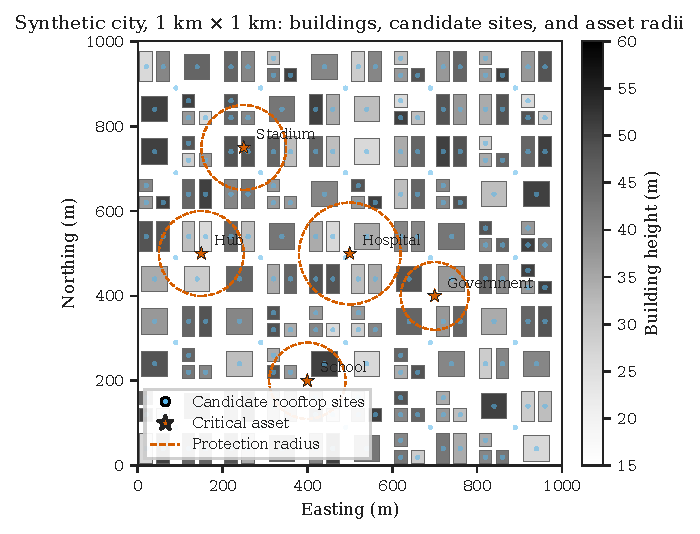
\includegraphics[width=0.92\textwidth]{figures/journal/fig_scenario_city.pdf}
  \caption{Synthetic planning scene. Gray polygons are buildings shaded by height. Blue points are candidate sensor sites. Orange stars and dashed circles are the five critical assets and their protection radii used to build the threat map.}
  \label{fig:scenario_city}
\end{figure*}

Planning floors used for post-filtering: \(M_{wp,coop}\geq0.90\), \(M_{wp,noncoop}\geq0.35\) (practical) and stretch \(0.90/0.50\).

\textbf{Seeds.} The city front is rerun with seeds 0, 1, and 2 at the same budget. For each seed we report the hypervolume of the 3-objective front and the cheapest member with \(M_{wp,coop}\geq0.85\) and \(M_{wp,noncoop}\geq0.35\), summarized as minimum, median, and maximum. Hypervolume is computed exactly with reference point \((0,0,\$700\mathrm{k})\), coverage in \([0,1]\) and CapEx normalized by \$700k.

\textbf{Airways.} Three stored solutions from the city front (cheapest with \(M_{wp,coop}\geq0.80\); cheapest with \(0.85/0.35\); best non-cooperative) are re-evaluated per airway layer at 20, 45, and 65\,m. Each layer reports threat-weighted \(M_{wp}\) restricted to that layer. No optimizer is run for this analysis.

\subsection{Airport SJC (split fronts)}

Real OSM airport scene with runway exclusion. Split optimization runs \texttt{coop\_only} then \texttt{noncoop\_only} (\texttt{--split-objectives}) so dark-target cost is not hidden inside a cooperative optimum. Budget: resolution 40\,m, population 24, 12 generations.

\subsection{Avenida Paulista}

Real OSM corridor (6,389 buildings, 93 rooftop sites, two critical assets) with dual-layer objectives and \$15k site activation. Journal budget: resolution 30\,m, population 40, 20 generations, checkpointing enabled (\texttt{configs/paper\_rerun\_paulista\_journal.json}).

\subsection{Analysis pipeline}

Each run emits Pareto JSON, hypervolume, convergence plots, LoS-aware overview maps, flight-level \(M_c\), and cost-vs-threshold curves. Dual-layer fronts additionally emit coop$\times$noncoop target plots; \texttt{tools/select\_requirement\_solutions.py} reports cheapest feasible members under stated floors.

\subsection{Control A --- small-$n$ oracle}
\label{sec:protocol_oracle}

To bound GA quality where enumeration is feasible, we crop the synthetic city to \(n\in\{8,10,12\}\) candidate sites and place \(k\in\{3,4,5\}\) sensors. All methods use the \emph{same} precomputed ray-traced \(P_D\) grids and classic coverage \(M_c\) at threshold \(0.8\) (resolution 40\,m). Comparators: Exhaustive (full site$\times$type enumeration when \(\leq120\)k combinations; otherwise site-exhaustive with type sampling), Greedy (marginal \(M_c\)), Random (matched budget samples), and a fixed-$k$ \(M_c\)-maximizing GA labeled NSGA-II* (5 seeds). We report \(M_c\), gap \(\Delta M_c = M_c^{\mathrm{oracle}}-M_c^{\mathrm{method}}\), and oracle wall time. This control does \emph{not} transfer optimality guarantees to city-scale fronts.

\subsection{Control B --- matched-budget modality ablation}
\label{sec:protocol_ablation}

At hardware CapEx budgets \(\{\$31\mathrm{k},\$76\mathrm{k},\$150\mathrm{k}\}\) on the same cropped synthetic geometry, we gate search to RF-only, Acoustic-only, EO-only, Radar-only, and Heterogeneous (all types) and report best achievable classic \(M_c\). Heterogeneity is claimed only when it wins at equal CapEx; lean RF wins are reported honestly.

\subsection{Control C --- dual-layer CapEx ablation}
\label{sec:protocol_dual_ablation}

Control~C repeats the matched-budget gates under threat-weighted dual-layer metrics \(M_{wp,coop}\) and \(M_{wp,noncoop}\) (same ray-tracer and five critical assets as the city dual-layer runs). Budgets \(\{\$31\mathrm{k},\$76\mathrm{k},\$150\mathrm{k},\$320\mathrm{k}\}\); \$320k matches the practical joint-floor CapEx band. Control~C is run twice: with hardware-only budgets, and with budget = hardware + \$15k per occupied site (each sensor occupies its own site). The heterogeneous gate includes every single-modality pack, so it can only tie or beat them up to site-sampling noise. For each modality$\times$budget we report (i)~the best-coop solution and its companion noncoop, and (ii)~the best-noncoop solution and its companion coop. Heterogeneity is claimed for a layer only when it wins that layer at equal CapEx.
